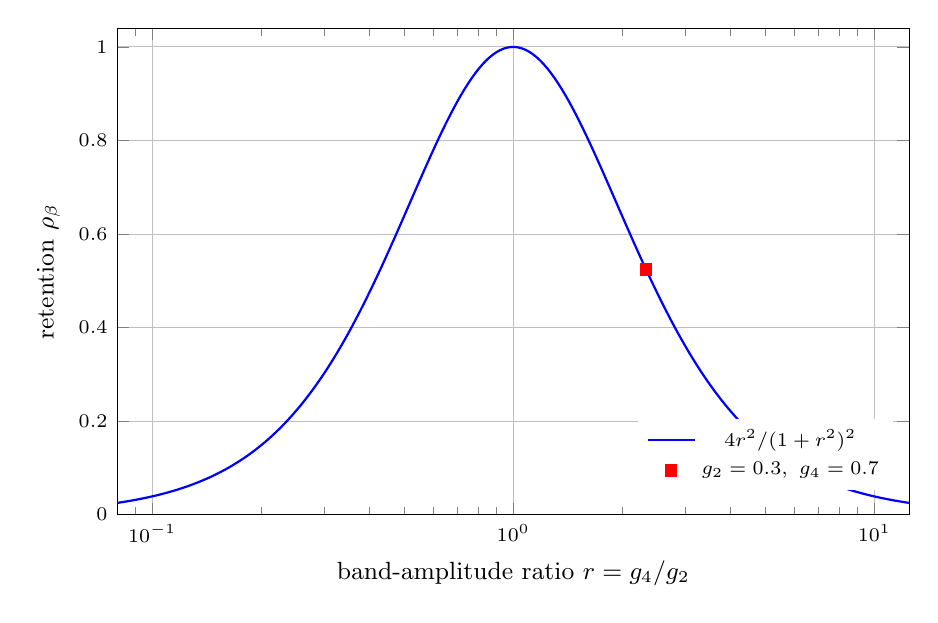
\begin{tikzpicture}
\begin{axis}[
 width=0.96\columnwidth,height=0.64\columnwidth,
 xmode=log,xmin=0.08,xmax=12.5,ymin=0,ymax=1.04,
 xlabel={band-amplitude ratio $r=g_4/g_2$},ylabel={retention $\rho_\beta$},
 grid=major,legend style={font=\scriptsize,draw=none,at={(0.98,0.05)},anchor=south east},
 tick label style={font=\scriptsize},label style={font=\small}]
\addplot[blue,thick,domain=0.08:12.5,samples=220] {4*x^2/(1+x^2)^2};
\addlegendentry{$4r^2/(1+r^2)^2$}
\addplot[only marks,mark=square*,red] coordinates {(2.3333333333,0.5243757431629014)};
\addlegendentry{$g_2=0.3,\ g_4=0.7$}
\end{axis}
\end{tikzpicture}
